\documentclass[12pt, a4paper]{report}
% for guidance, see phd_work/mnras_guide.pdf
%\setlength\parindent{0pt}

\usepackage[english]{babel}
\usepackage[utf8x]{inputenc}
\usepackage[T1]{fontenc}

%\documentclass[useAMS,usenatbib]{mn2e}
\newcommand{\aap}{A\&A}
\newcommand{\araa}{ARAA}
\newcommand{\mnras}{MNRAS}
\newcommand{\apjl}{ApJL}
\newcommand{\apjs}{ApJS}
\newcommand{\apj}{ApJ}
\newcommand{\aj}{ApJ}
\newcommand{\nat}{Nature}
\newcommand{\pasa}{PASA}
\newcommand{\pasj}{PASJ}
\newcommand{\pasp}{PASP}
\newcommand{\aapr}{A\&AR}
\newcommand{\procspie}{Proc. SPIE}
\newcommand{\apss}{Ap\&SS}
%\newcommand{\rsquo}{`}

\usepackage{graphicx}
%\usepackage{braket}
\usepackage[english]{babel}
\usepackage{upgreek}
\usepackage{graphicx}
\usepackage{float}
\usepackage{natbib}
\usepackage{amsmath}
\usepackage{amssymb}
\usepackage{tabularx,ragged2e,booktabs,caption}
\usepackage{graphicx} % for images
\usepackage[font=small]{caption}
\usepackage{setspace}
\usepackage{epstopdf}
\usepackage{subcaption}
\usepackage{url}

% ALW edit: FORMAT FOR INCLUDING PDF IMAGES!!!
% for guidance, see phd_work/grfguide.pdf
%\includegraphics[<options>]{filename.pdf}


%%%%%%%%%%%	Page layout settings that follow JMU regulations     %%%%%%%%%%

\setlength{\hoffset}{0mm}
\setlength{\oddsidemargin}{0mm}
\setlength{\evensidemargin}{0mm}

\setlength{\voffset}{-10mm}
\setlength{\topmargin}{0mm}
\setlength{\headheight}{10mm}
\setlength{\headsep}{10mm}

\setlength{\textheight}{220mm}
\setlength{\textwidth}{155mm}

\setlength{\columnsep}{10mm}
\setlength{\marginparsep}{0mm}
\setlength{\marginparwidth}{0mm}
\setlength{\footskip}{20mm}

\setlength{\parindent}{0.3in} % Size of indent at the start of a new paragraph - originally 0.0in
\setlength{\parskip}{0.0in} % Spacing between paragraphs - originally 0.1in

\usepackage[hang,splitrule]{footmisc}

\addtolength{\footskip}{0.5cm}
\setlength{\footnotemargin}{0.3cm}
\setlength{\footnotesep}{0.4cm}

\makeatletter
\let\splitfootnoterule=\pagefootnoterule
\makeatother



\begin{document}

\chapter{Methodology}
\section{Software used}
To generate the predicted stellar flux, the ATLAS9 model stellar atmosphere code \citep{1993KurCD..13.....K} was used to produce monochromatic fluxes for a series of wavelengths at short**** intervals, ranging from ****nm to ****nm.  Table 1 of \cite{2004astro.ph..5087C} contains precise details of the coverage in $T_{\textnormal{eff}}$-log($g$) parameter space, while a brief summary  of the limits of the space is listed in Table \ref{atlas9_input}. Four input metallicities were used for ATLAS9, at values of [Fe/H] = -2, -1, 0 and 0.5, covering the metallicities of most observed globular and open clusters.

The tables of bolometric corrections were generated using a FORTRAN 77 code incorporating the steps described in Section \ref{BC_theory}, inputs with data tables describing the response functions of all three filter systems at the same wavelengths as the ATLAS9 model atmosphere tables. The number of BC tables for each stellar metallicity value equal to the total number of ATLAS9 ($T_{\textnormal{eff}}$, log($g$)) combinations available.

Once the bolometric correction tables were produced, all subsequent processes were written in Python 2.7 in the form of IPython notebooks. The repository containing all data, plots and programme codes for this project can be found at \protect\url{https://github.com/AlexlwAstro/phd_work}.

\begin{table}
\begin{center}
\begin{tabular}{cccc}
\hline
%\multirow{2}{*}{System} & \multirow{2}{*}{Filter} & \multirow{2}{*}{$A_{1}$ function} & \multicolumn{3}{c}{$A_{1}$ coefficients} \\ \cline{4-6}
%\textbf{Filter} \\
Parameter / unit & Minimum & Maximum & Number of values \\
\hline
$T_{\textnormal{eff}}$ / K & 3500 & 50000 & 76 \\
log( $g$ / cm s$^{-2}$) & 0.0 & 5.0 & 11 \\
$\textnormal{[Fe/H]}$ & -2.0 & 0.5 & 4 \\
\hline
\end{tabular}
\caption{Ranges for the input parameters for ATLAS9 atmospheric models}
\label{atlas9_input}
\end{center}
\end{table}


The isochrones used were generated using the latest Bag of Stellar Tricks and Isochrones (BaSTI) web interface \citep{2004ApJ...612..168P}\citep{2018ApJ...856..125H}. The filter systems whose throughput data were employed by BaSTI to generate the fluxes for the isochrones were ACS, WFC3 and Gaia-DR2. It should be noted that the WFC3 isochrone output does not include flux magnitudes for the F300X filter.

\section{Extinction data}
When calculating the bolometric corrections, the reference values taken as the apparent magnitude for Vega were:

\begin{enumerate}
\item $m_{X}^{0} = 0.03$ for the Gaia filters
\item $m_{X}^{0} = 0.00$ for the Hubble WFC3 filters
\end{enumerate}

together with $M_{\textnormal{bol},\odot} = 4.75$ for the solar absolute magnitude. Equation \ref{CCM_general}, with the different wavelength regimes for $a(x)$ and $b(x)$ described by \cite{1989ApJ...345..245C}, was used with the $A_{V}$ calibration values to simulate the extinction parameter in Equation \ref{BC_extinc}. $R_{V}$ was set to a value of 3.1, the standard value for the diffuse interstellar medium. The integration was carried out by iteratively adding the integrand results at regular small wavelength intervals. The non-zero calibration value of $A_{V} = 1$ was chosen, as this allows for significant changes in $A_{X}/A_{V}$ from Equation (\ref{BCs_diff}), while also being close enough to zero to avoid significant changes in $A_{X}/A_{V}$ due to the Forbes effect \citep{2008PASP..120..583G}.

To generate extinction-coefficient ratios $A_{X}/A_{V}$ from the bolometric correction data, Equation \ref{BCs_diff} was used to****

\begin{figure}[h]
\begin{center}
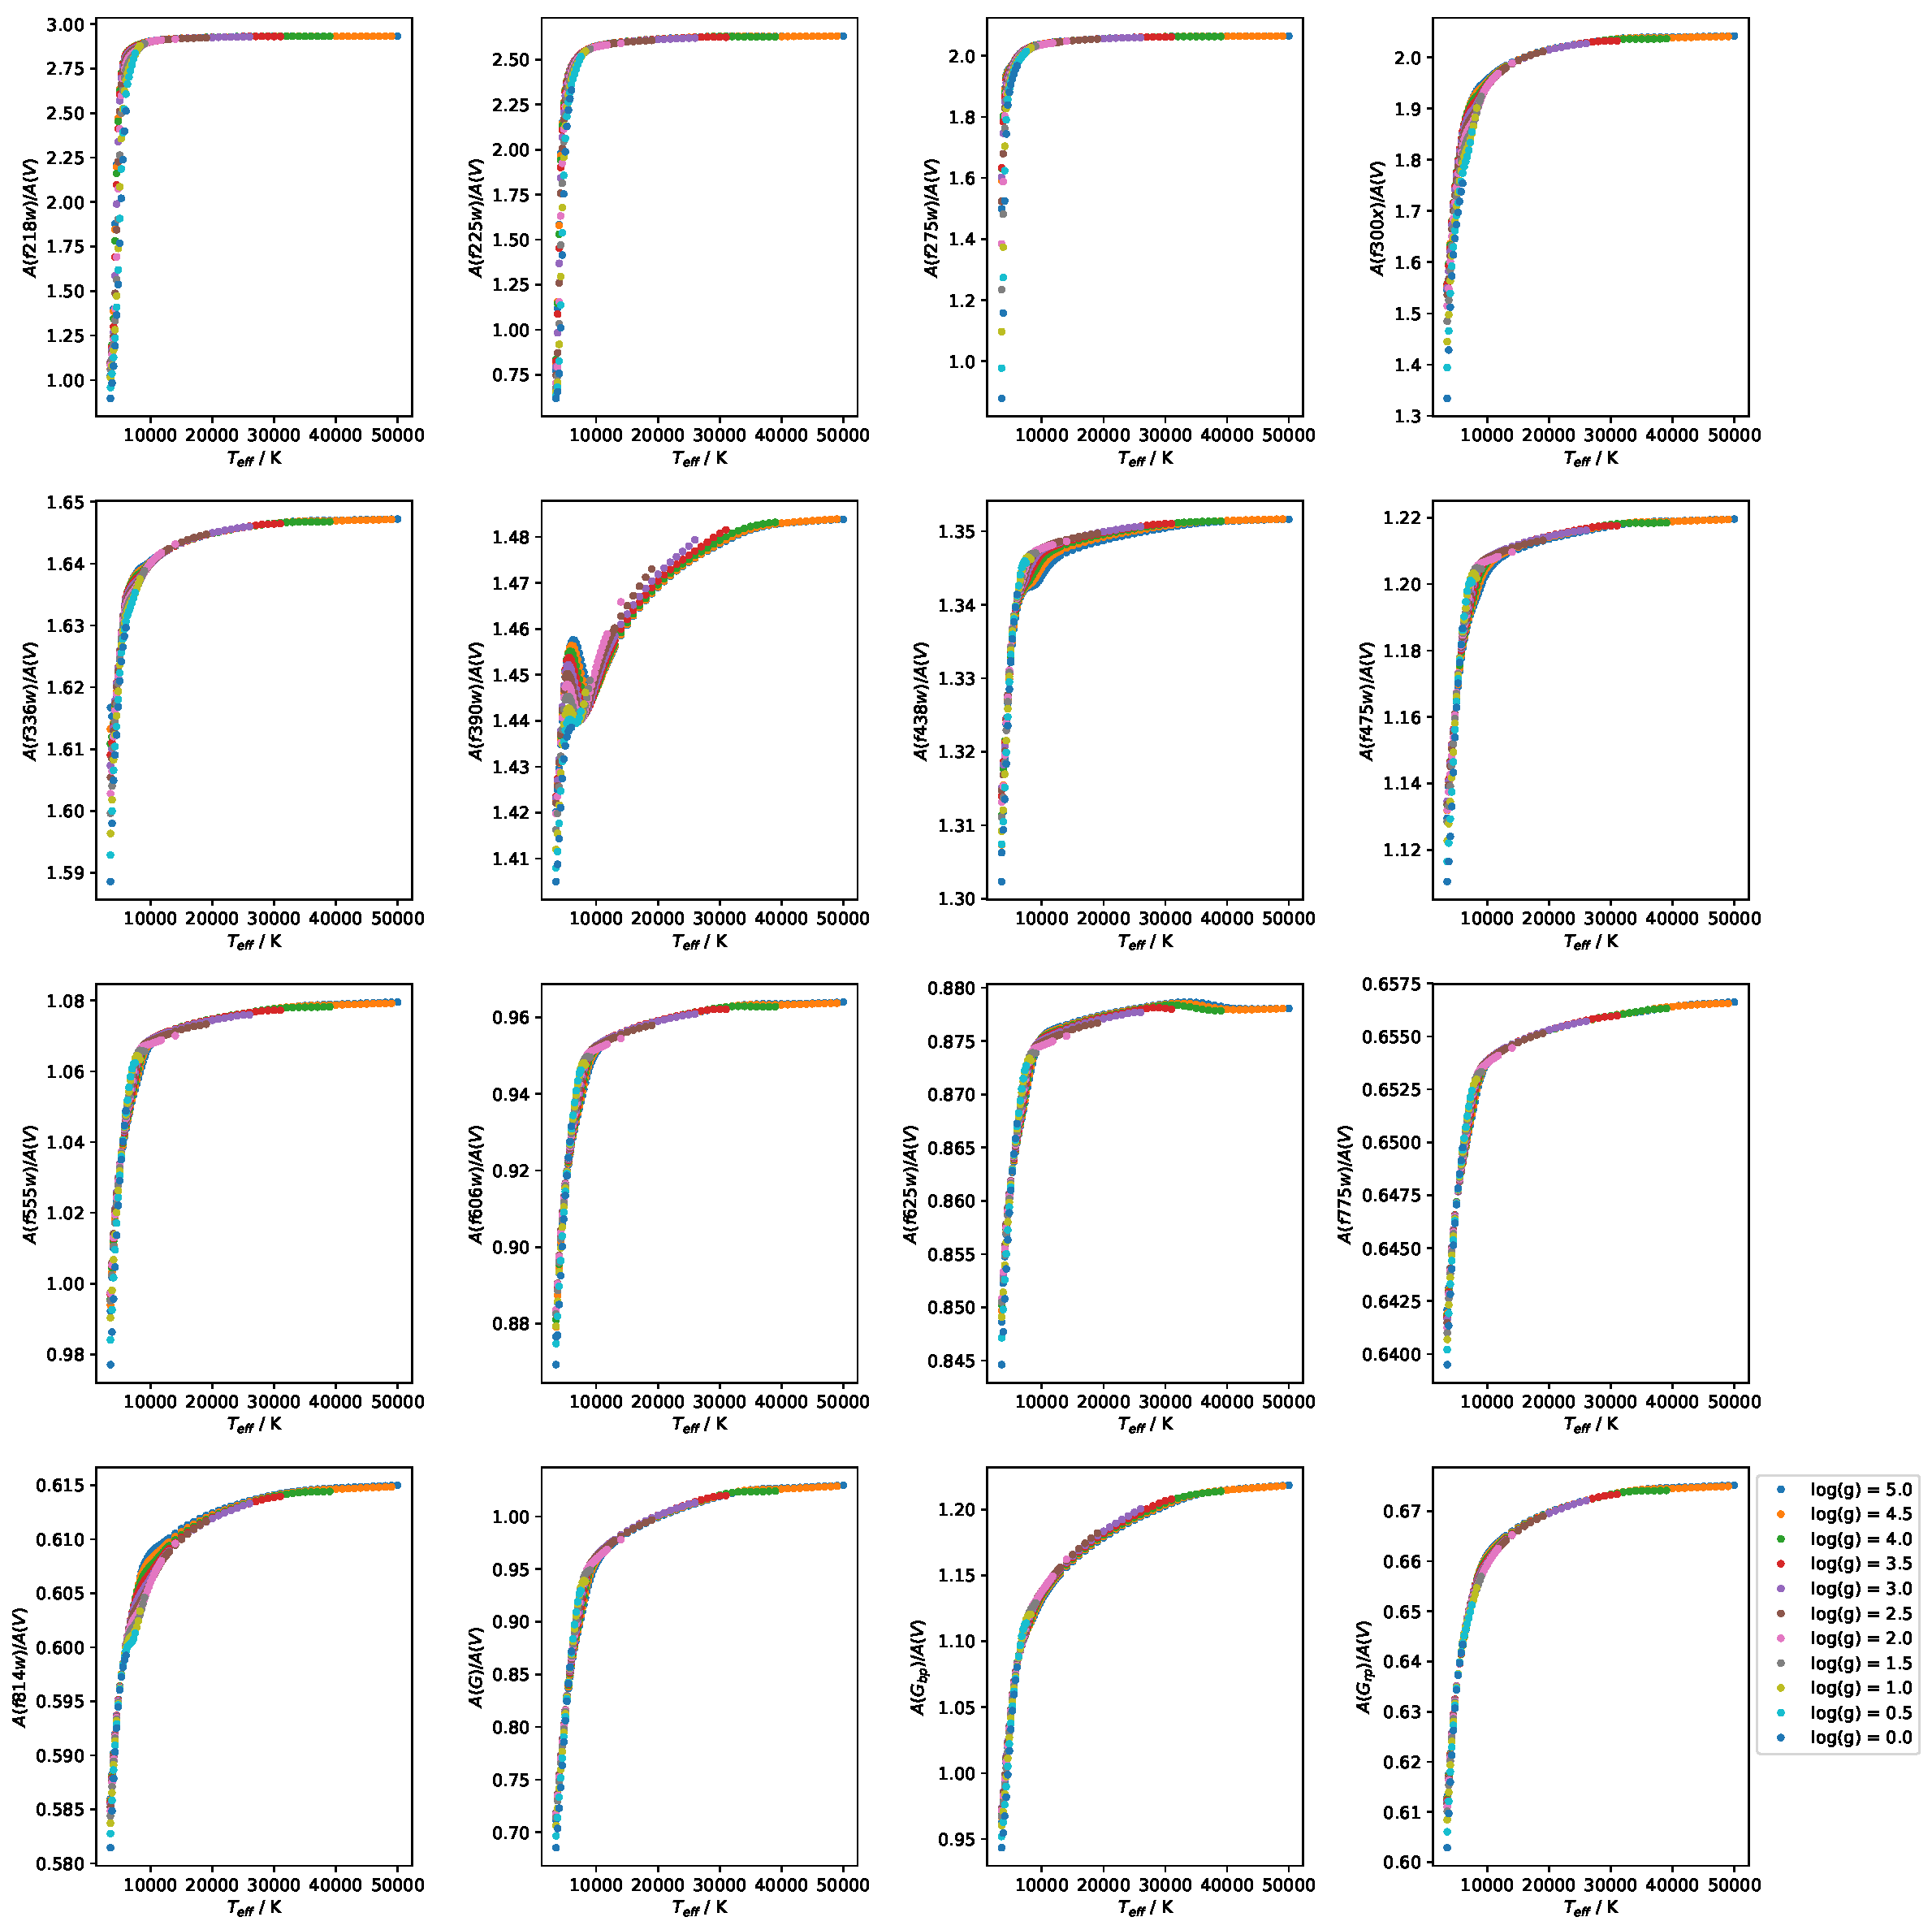
\includegraphics[scale=0.3]{../just_full_data/comb/AHub_FeHm2p0_just_Teff_fit_plot_dots.pdf}
\caption{****Monochromatic flux of a black body for different stellar effective temperatures. The black dashed lines mark the approximate limits of the visible part of the EM spectrum. The green curve represents the distributed of the maxima for the other curves.}
\label{Ax/Av data FeH=-2}

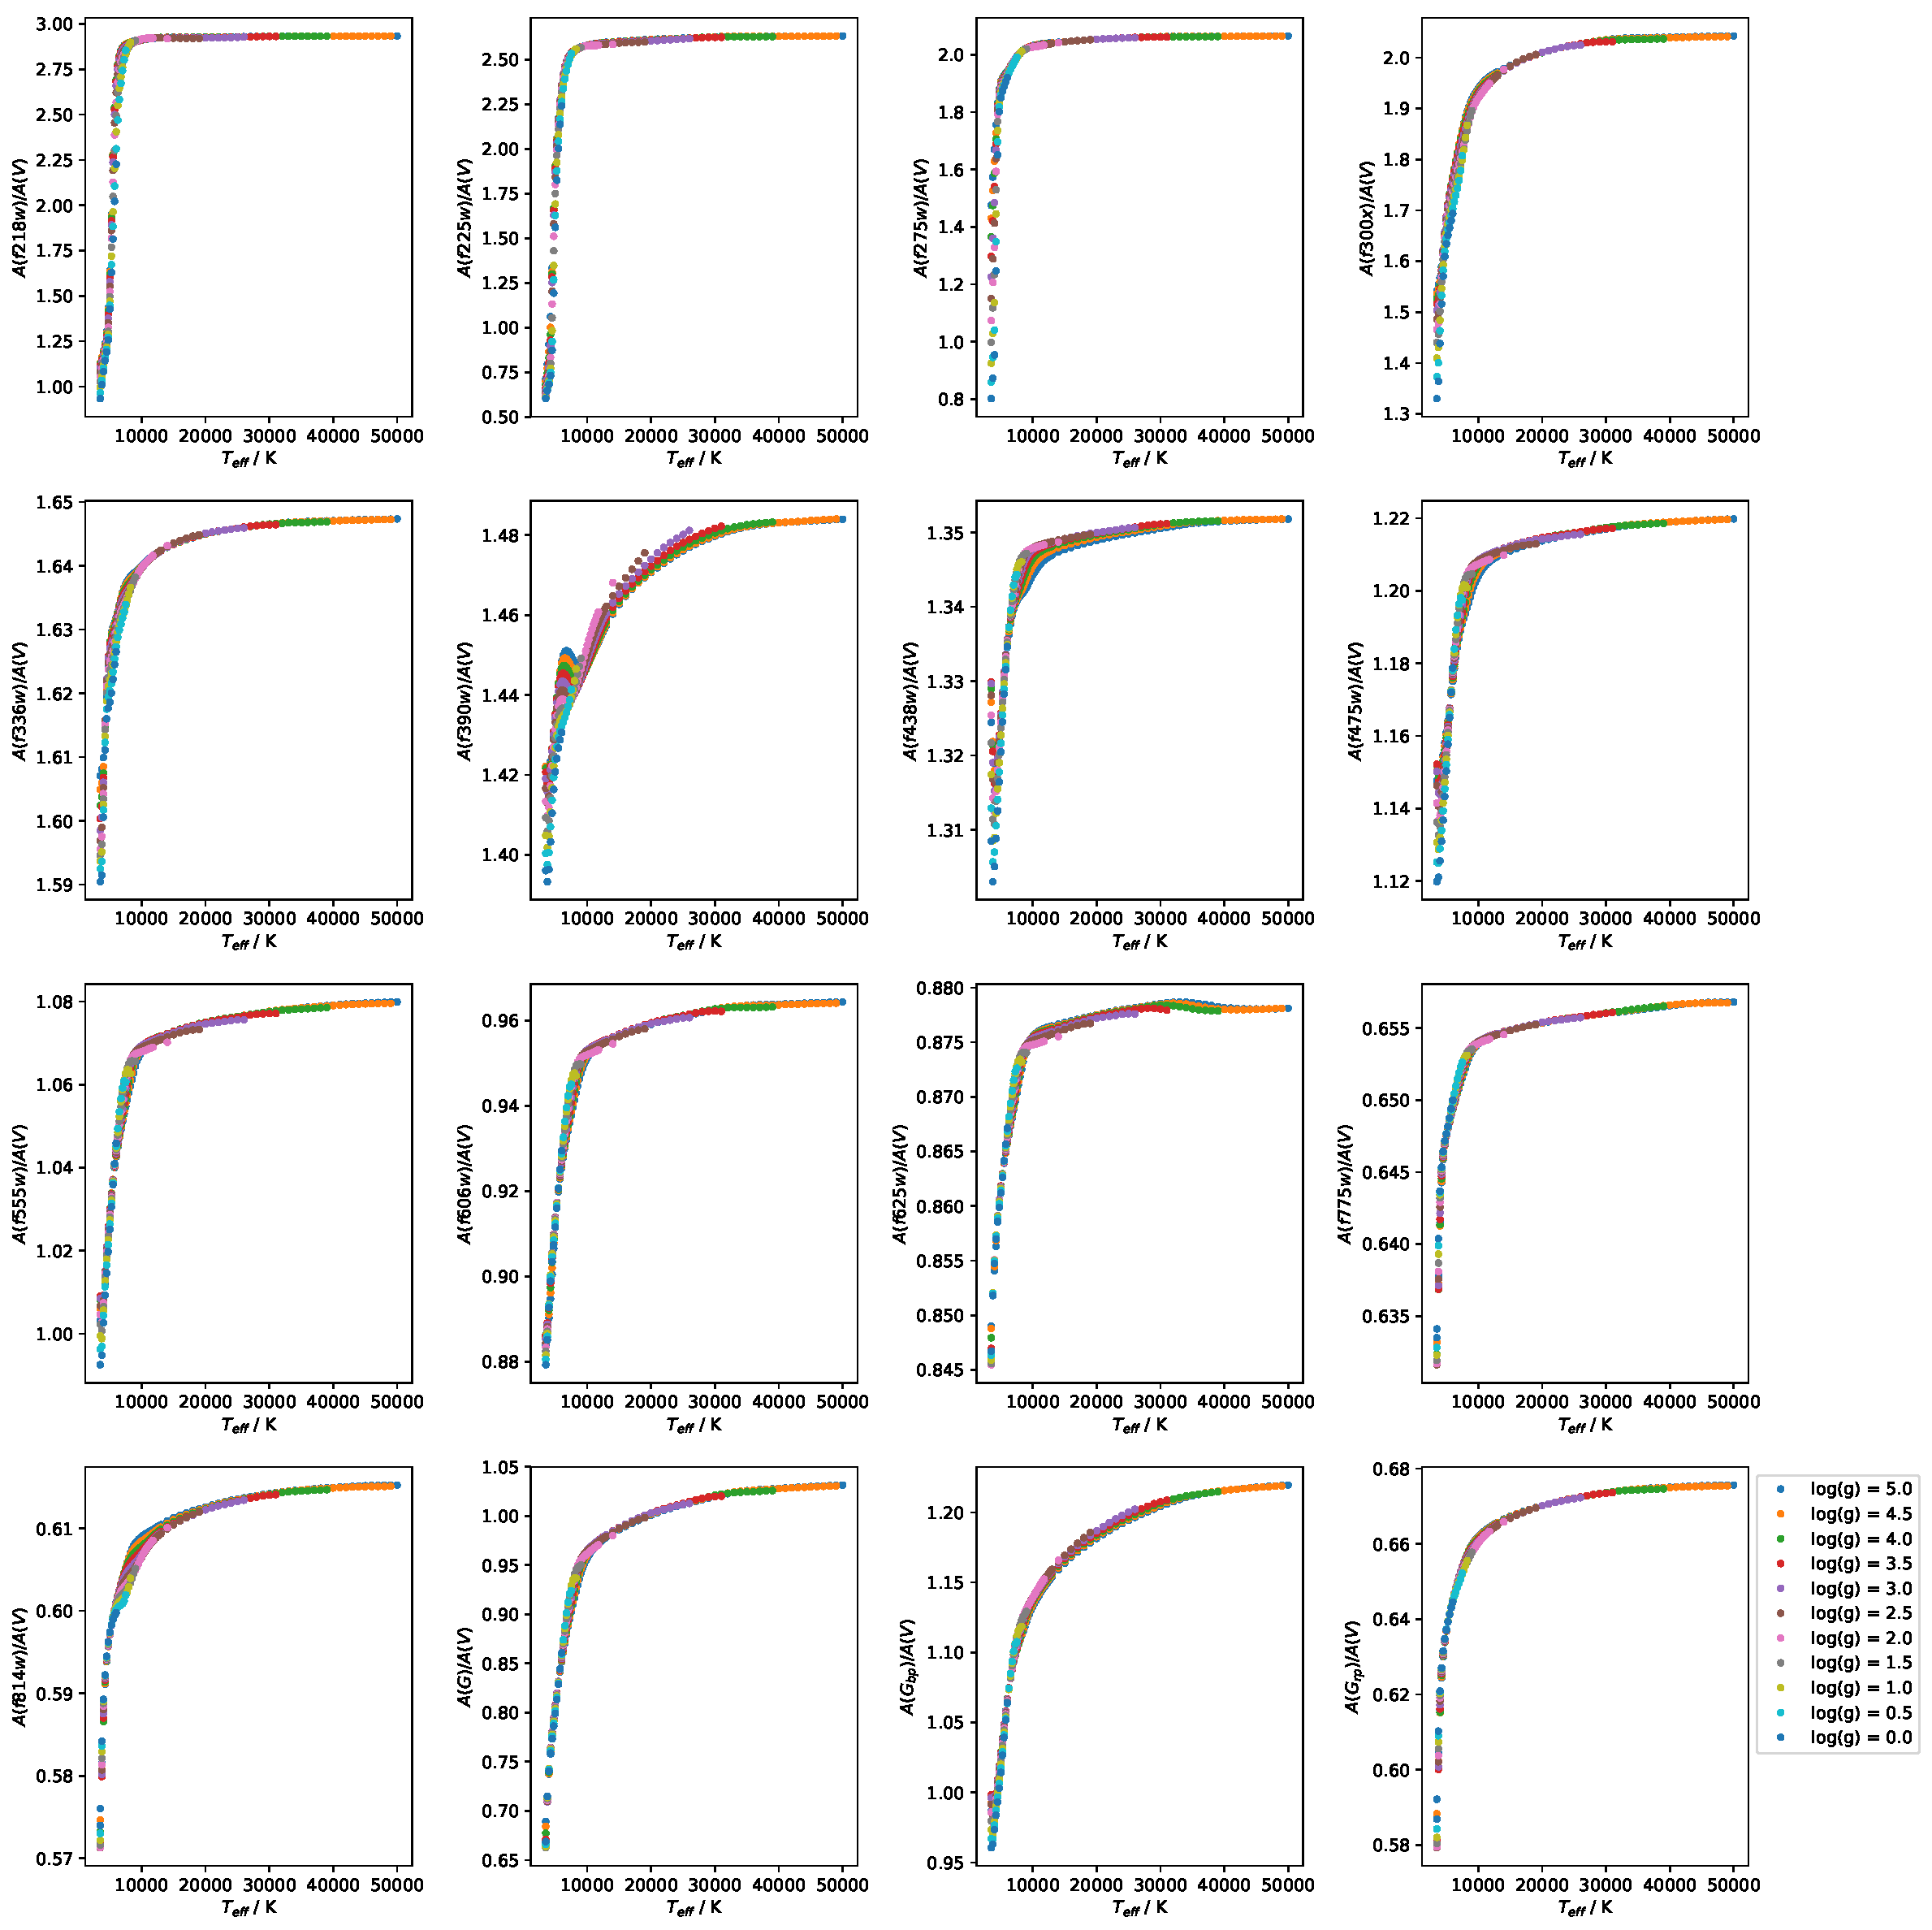
\includegraphics[scale=0.3]{../just_full_data/comb/AHub_FeH0p0_just_Teff_fit_plot_dots.pdf}
\caption{Solar metallicity}
\label{Ax/Av data FeH=0}
\end{center}
\end{figure}

\begin{figure}[h]
\begin{center}
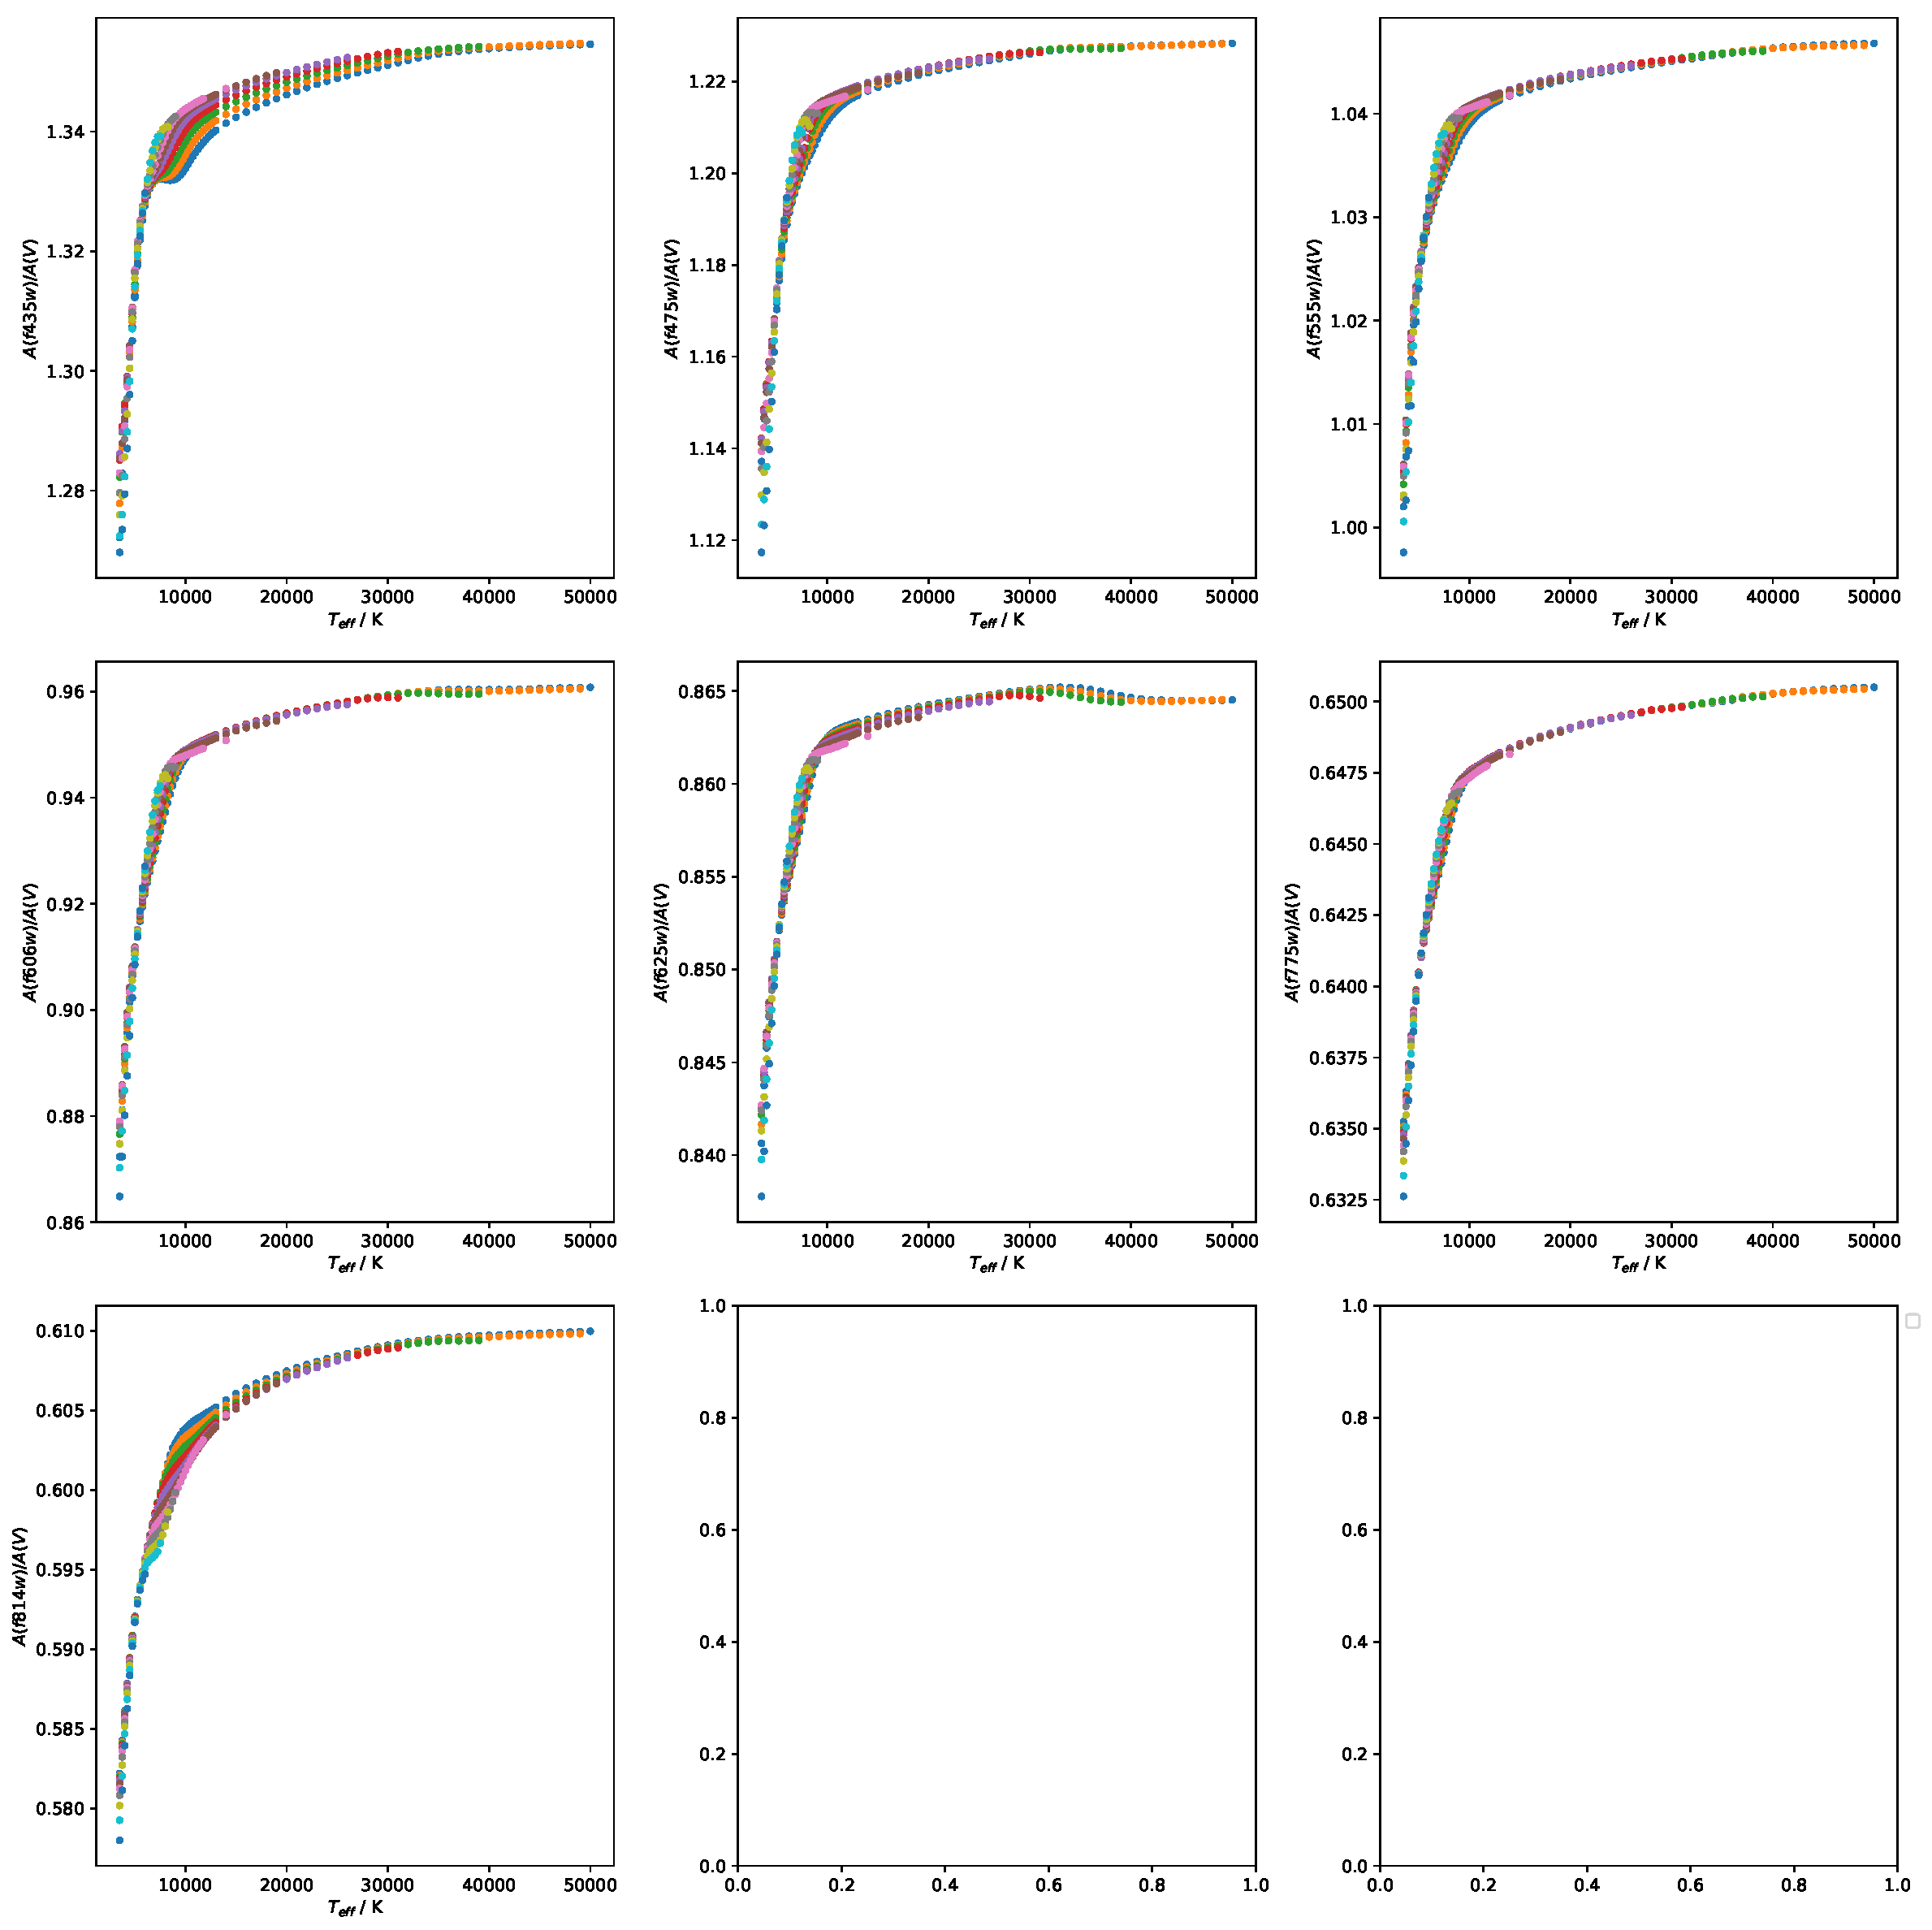
\includegraphics[scale=0.3]{../just_full_data/ACS/AHub_FeHm2p0_just_Teff_fit_plot_dots.pdf}
\caption{****Monochromatic flux of a black body for different stellar effective temperatures. The black dashed lines mark the approximate limits of the visible part of the EM spectrum. The green curve represents the distributed of the maxima for the other curves.}
\label{Ax/Av data FeH=-2}

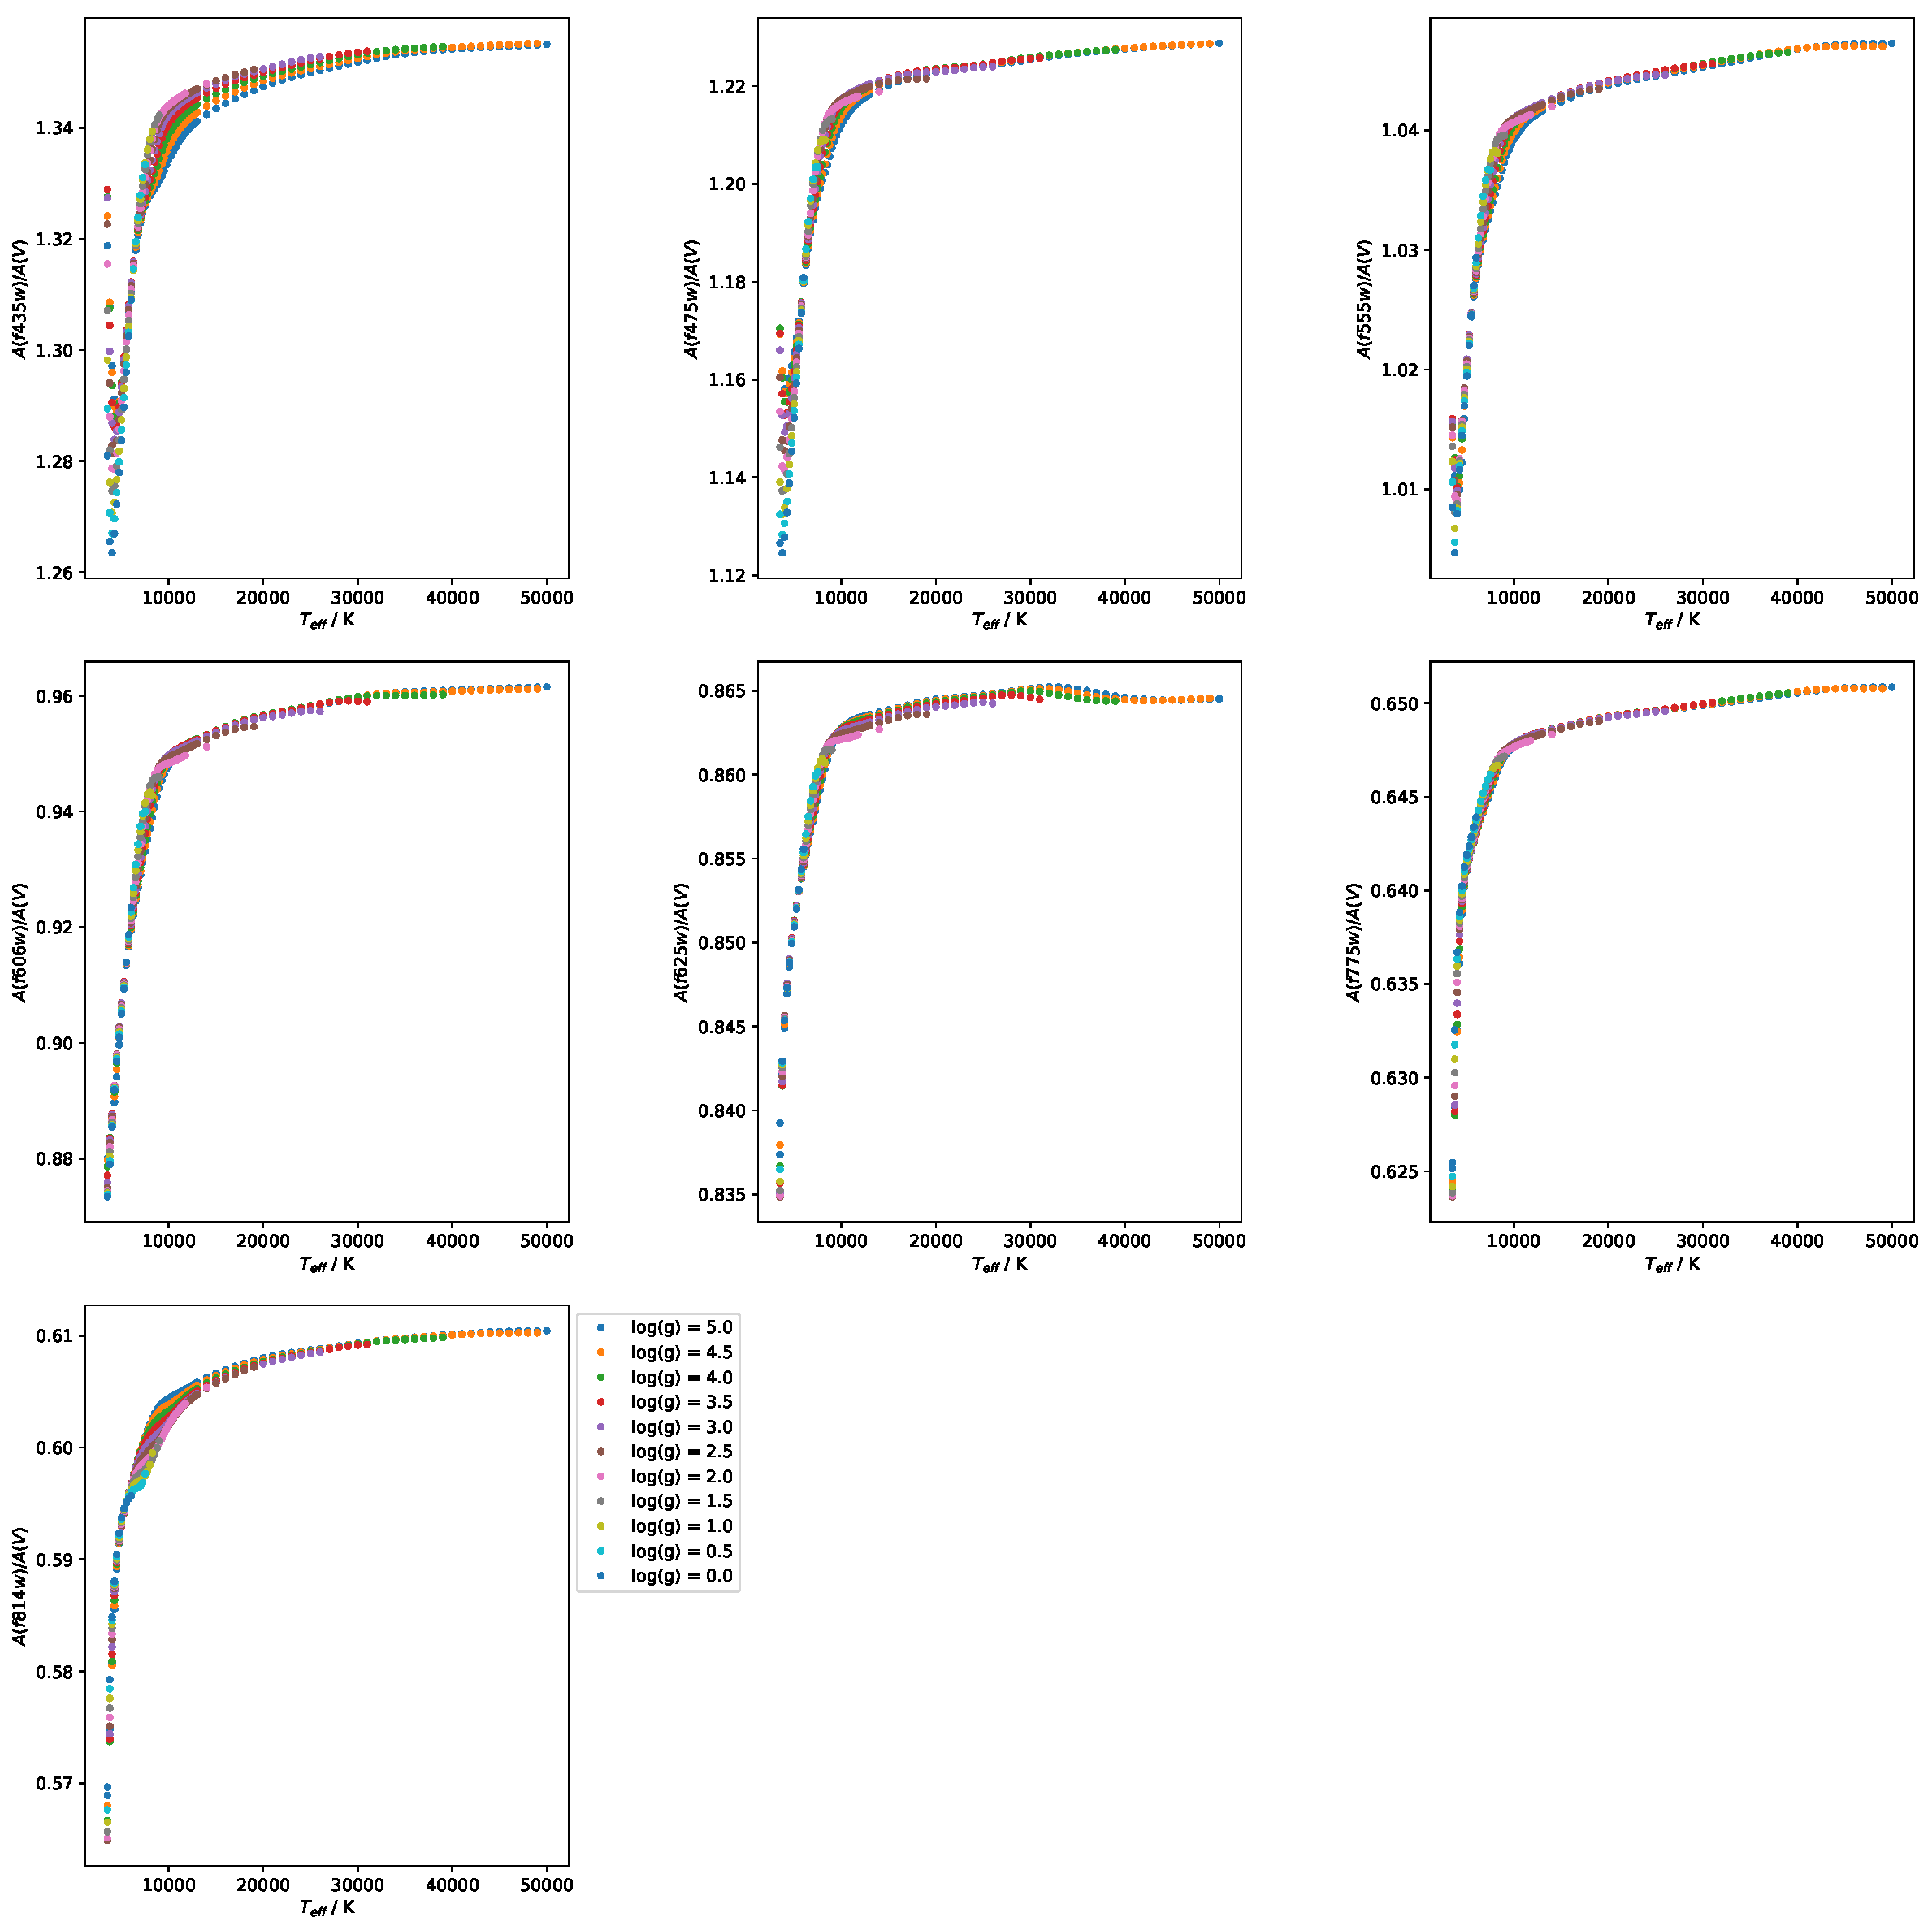
\includegraphics[scale=0.3]{../just_full_data/ACS/AHub_FeH0p5_just_Teff_fit_plot_dots.pdf}
\caption{Solar metallicity}
\label{Ax/Av data FeH=0}
\end{center}
\end{figure}

\section{Finding \& fitting functions} \label{find_fit}
A property found in the data for some filters, more pronounced at higher metallicity but with a possible slight dependence on surface gravity, is the tendency of the gradient of $A_{X}/A_{V}$ with increasing $T_{\textnormal{eff}}$ to become significantly less positive at the lowest temperatures in the data, typically 4000K and below. The spread in $A_{X}/A_{V}$ values for different log($g$) is between 0.02 and 0.04, with a linear progression from log($g$) = 5.0 at the lowest end to log($g$) = 0.0 at the highest. In some filters, at the highest metallicity employed ([Fe/H] = 0.5), this phenomenon causes the gradient to become significantly negative, reversing the trend everywhere else in the data, including for the same filters at lower metallicity. Due to the shape of the resulting point-to-point line in these axes, it has been dubbed the ``tail-flick'' phenomenon. In filters for which the tail-flick resulted in a negative gradient in the $T_{\textnormal{eff}}$-$A_{X}/A_{V}$ plane, the data points impacted by the phenomenon were ignored during fitting. The phenomenon was treated as an artefact from the numerical integration required for Equation \ref{BC_extinc}. This was due to the physical infeasibility of a cooler star experiencing a higher extinction $A_{X}$ for a globally-constant $A_{V}$ value and metallicity, as was assumed for data in each BC table.

In order to find usable functions without running into issues with degeneracy between coefficients, the three input stellar parameters prioritising which parameters to model first, before expanding the function to include parts modelling the impact of other parameters and their associated coefficients. Too many coefficients created errors that were significantly greater in degenerate coefficients than in non-degenerate ones. This would obscure any useful information about the validity of the form of the function in question.

The monochromatic flux of a black body can be calculated as the total area under the curve described by the Planck function per unit wavelength/frequency as a function of wavelength/frequency. Since stellar emission spectra can be reasonably approximated by a black body emission with absorption lines, it can be seen from Equation\ref{Teff_def} that the greatest effect on stellar spectra, and therefore on the extinction coefficient, will come from effective temperature. Therefore, the initial functions to be fitted were simple analytical functions of $T_{\textnormal{eff}}$ only:

\begin{equation}
A_{\textnormal{pow}} (T_{\textnormal{eff}}) = a (T_{4})^{b} + c
\label{Teff_pow}
\end{equation}

\begin{equation}
A_{\textnormal{exp}} (T_{\textnormal{eff}}) = a \exp(b T_{4}) + c
\label{Teff_exp}
\end{equation}

where, as before, $T_{4} = 10^{-4} \times T_{\textnormal{eff}}$. The fitting operation was carried out on the data for solar metallicity ([Fe/H] = 0.0) and, because it gave the greatest number of $T_{\textnormal{eff}}$ data points, log($g$) = 5. This dataset will be referred to as the basic fitting data (BFD).

Casagrande comparisons****
Girardi****

For filters whose data could not support an accurate**** fit on this data or could not keep accuracy across all combinations of log($g$) and [Fe/H] using $A_{\textnormal{pow}}$ or $A_{\textnormal{exp}}$, more ****complicated functions were sought, including functions with dependences on $g$ and [Fe/H].
For these filters, several unsuccessful approaches were made before an acceptable function was found for each filter. These included:
\begin{itemize}
\item Using a polynomial fit for the BFD, for filter which could not be accurately described in the BFD in the first instance.
\item Fitting all the data in the ****parameter space in two steps, by fitting the residuals from the $A_{\textnormal{pow}}$ and $A_{\textnormal{exp}}$ fits to a new function with explicit variations in [Fe/H] and log($g$). The ****functions included second fittings of $A_{\textnormal{pow}}$ and $A_{\textnormal{exp}}$, damped-oscillator functions and oscillating power-law functions, among others. When fitted to the residuals, this meant an oscillation with amplitude decaying with increasing $T_{\textnormal{eff}}$
\end{itemize}


A more successful approach was to individually**** tailor the form of the function for each filter. All the available data for each filter was plotted, in multiple 2D and 3D axes, and the trends seen in the data were transcribed to find not only an overarching model template, akin to the status of $A_{\textnormal{pow}}$ and $A_{\textnormal{exp}}$, but also individual sub-functions, such as describing an exponential decay coefficient using a linear combination of log($g$) and [Fe/H] terms.
****Add other functions here!

For the four UV filters in WFC3, the final form for the overarching template for $A_{X}/A_{V}$ was a logistic function in $T_{\textnormal{eff}}$, shown in Equation \ref{A_logis_UV}. For a general logistic function in $T_{\textnormal{eff}}$, there are four principle parameters:
\begin{itemize}
\item The global maximum value, denoted in this case by $A_{max}$;
\item The global minimum value, $A_{min}$;
\item The exponential decay coefficient, $k$;
\item The $T_{\textnormal{eff}}$-coordinate of the sigmoid midpoint, in this case $T_{\textnormal{0}}$.
\end{itemize}

This form was chosen on the basis of its ability to model the low-$T_{\textnormal{eff}}$ change in gradient for these filters, which appears to be more significant in these filters than for others, as can be seen in Figures \ref{Ax/Av data FeH=0} and \ref{Ax/Av data FeH=-2}, even after accounting for the difference in scale between the maxima and minima in each filter. In particular, the $T_{\textnormal{eff}}$ gradient prior to the plateau appears to lead to an asymptote at lower, but still potentially-feasible temperatures. This issue is resolved by the change in gradient, which can be accurately modelled using a logistic curve, while also maintaining accuracy in modelling the gradient change during the transition to the plateau.

However, the problems regarding the significant changes in extinction ratios with surface gravity and metallicity required addressing. Therefore, upon inspection of the data over all combinations of both parameters, the logistic coefficients $T_{0}$ and $k$ were expressed as simple functions of $g$ and [Fe/H], shown in Equations \ref{T0_eq} and \ref{decay_const_eq}, respectively. Therefore, the overall function $A_{logis}$ is sensitive to all three input stellar atmosphere parameters, with effective temperature having the greatest effect and the effects of the other parameters dependent on the best-fit values of the relevant coefficients.

\begin{align}
T_{\textnormal{0}} &= a\log(g) + b\left(\frac{\textnormal{[Fe/H]}}{\left|\textnormal{[Fe/H]}\right|^{1/2}}\right) + c \label{T0_eq}\\
k &= d\log(g) + e\textnormal{[Fe/H]} + f \label{decay_const_eq}\\
A_{logis}(T_{\textnormal{eff}},g,\textnormal{[Fe/H]}) &= \frac{(A_{max}-A_{min})}{( 1 + \exp{(-10^{-4}k(T_{\textnormal{eff}}-T_{\textnormal{0}})) ) )}} + A_{min} \label{A_logis_UV}
\end{align}

In general, the longer the effective wavelength of a given filter throughput, the smaller the value of $A_{X}/A_{V}$. This conforms with the expectation resulting from the fact that the physical mechanisms causing extinction in the ISM preferential affect photons with shorter wavelengths.


\section{Isochrone data fitting}
To obtain isochrones from the BaSTI online database, the desired age range, initial metallicity and filter system must be specified. Therefore, the values of these quantities are shared by all stellar objects. For the stages in stellar evolution prior to the main-sequence turn-off, any changes in atmospheric metallicity are insignificant, due to the factors discussed in Section \ref{stel_evol}.

The output from the BaSTI database for each model stellar object gives the model's initial mass and current mass (i.e. after a time equal to the isochrone age), together with the logarithms of the stellar luminosity in solar units ($\log(L/L_{\odot})$) and of the effective temperature in K ($\log(T_{\textnormal{eff}})$), followed by the absolute magnitudes (with zero extinction) of the object in each filter of the system. To derive the surface gravity $g$, we must combine Equation \ref{Teff_def}, to derive the stellar radius, and Equation \ref{gravity_def}. Equation \ref{gravity_LT_calc} shows the resultant definition of $g$:

\begin{equation}
\label{gravity_LT_calc}
g = \frac{4 \pi G M_{*} \sigma_{\textnormal{SB}} T_{\textnormal{eff}}^{4}}{L_{*}}
\end{equation}

After this had been completed, each object had a co-ordinate in ($T_{\textnormal{eff}}$, log($g$)) parameter space, plus the metallicity of the overall isochrone model. The functions described in Section \ref{find_fit} were then applied to the dataset of stellar objects, producing values of $M_{\textnormal{eff},X}$ for each filter for all objects.

\begin{table}
\begin{center}
\begin{tabular}{ccccc}
\hline
Isochrone & $T_{\textnormal{eff}}$ & $T_{\textnormal{eff}}$ & $\log(g)$ & $\log(g)$ \\
(Age/Myr , [Fe/H]) & minimum & maximum & minimum & maximum \\
\hline
500,0.002 & 2870 & 9640 & 0.886 & 5.137 \\
1000,0.002 & 2824 & 8035 & 1.608 & 5.184 \\
5000,-1.049 & 3118 & 7112 & 0.456 & 5.318 \\
10000,-1.049 & 3086 & 6412 & 0.286 & 5.332 \\
\hline
\end{tabular}
\caption{Ranges of effective temperature and surface gravities in selected BaSTI isochrones}
\label{variable_ranges}
\end{center}
\end{table}

****However, the filter magnitudes in the photometric data were the original apparent magnitudes, not absolute magnitudes. Therefore, to match the attributes**** of the observational and isochrone datasets, it was necessary to correct the observational fluxes**** for distance and add extinction to the isochrone data, ****as is done by observers. Thus, we were comparing the $M_{ext,X}$ values for the isochrones and the observational data.

****Girardi CMD comparison

****The errors in the parallax data for objects assigned to NGC 6793 were significant, particularly for stars in the lower main-sequence - understandably, since they are the faintest objects in the data and therefore are more difficult to track against the bakcground light sources. This leads to errors in the predicted $M_{ext,X}$ magnitudes, which is calculated by rearranging Equation \ref{distance_modulus}. ****The significance of the parallax errors in the main sequence is such that even when assuming no errors in the observed fluxes from the photometric filters, any differences between isochrones with similar parameters are rendered insignificant.

Since the table for photometric fluxes did not include photometric errors, the parallax errors alone accounted for the total error in the calculated $M_{ext,X}$. Therefore, the errors on the flux measurements  were exactly equal in all filters for a given star. The errors on the ($G_{\textnormal{bp}}-G_{\textnormal{rp}}$) color index were calculated as standard, by adding the individual filter errors in quadrature, giving the color errors which were a factor of $\sqrt{2}$ greater than those for the individual filter fluxes.


When comparing the two approaches to extinction, in order to test for any differences in projected isochrone age via the MSTO, a range of ages must be considered. A ``primary'' age was utilised as the true cluster isochrone age. This primary isochrone was subjected to both the function-based and standard extinction approaches. Two isochrones with ages equidistant from the primary were subjected to the standard approach only. All four of the resulting $M_{ext,X}$ isochrones were plotted together in the four chosen CMD axes, together with the original (zero-extinction) isochrone for visual reference.

As can be seen in the data****, in all the filters studied in this project, above $T_{\textnormal{eff}} \approx$ 12000-15000 K, the values of $A_{X}/A_{V}$ are constant or near-constant as a function of all three input parameters, reflected in the choice of decay functions for fitting the data****. This will be referred to henceforth as the ``extinction plateau''.

This**** was repeated for two values of the standard treatment. Both were extracted from the ATLAS9 data tables, for a log($g$) value of 5.0, thus**** representing a main-sequence star, highly desirable when comparing MSTO positions. The ATLAS9 metallicity chosen for these values**** was that which best matched the metallicity of the isochrone to which the coefficient was applied, ****which we will call [Fe/H]$_{CM}$. The first value was equal to $(A_{X}/A_{V})_{plat} = (A_{X}/A_{V})(T_{\textnormal{eff}} = 50,000\textnormal{K},\log(g) = 5.0,[Fe/H]_{CM})$, and the second was equal to  $(A_{X}/A_{V})_{MS} = (A_{X}/A_{V})(T_{\textnormal{eff}} = 5,000\textnormal{K},\log(g) = 5.0,[Fe/H]_{CM})$. This was done to reflect the fact that, on one hand, the assumption of a constant extinction coefficient is valid in the plateau region and, on the other, given the position of the MSTO in terms of stellar model $T_{\textnormal{eff}}$ values, it would be more prudent to ensure that the upper main sequences resulting from both approaches to extinction coincide in the CMD, making it easier to see disagreements in the turn-off ages****. For each of these plots****, $A_{V}$ was fixed at a value of 1.0.

For the open cluster NGC 6793, the isochrone fitting was done by eye. Using the values of $E(B-V)$ and age from \cite{2018A&A...616A..10G}, a standard-case isochrone was derived, assuming a diffuse ISM (i.e., $R_{V} = 3.1$). This was tested for both $(A_{X}/A_{V})_{MS}$ and $(A_{X}/A_{V})_{plat}$. The fitting process was carried out in sequential stages:
\begin{enumerate}
\item First, the upper main sequence of the function-based**** extinction isochrone was fitted to that of the standard-case isochrone by varying the value of $A_{V}$ used for the function-based**** extinction coefficient.
\item Next, the age of the FBE*** isochrone was varied to match the observed turn-off location in the NGC 6793 data as far as possible.
\item Finally, the FBE isochrone metallicity was varied in an attempt match the observed lower main-sequence.
\end{enumerate}

The isochrone with the resulting parameters were then plotted alongside the standard-case isochrones using both $(A_{X}/A_{V})_{MS}$ and $(A_{X}/A_{V})_{plat}$. The resulting curves were compared to each other for accuracy with respect to the observational data.

\bibliographystyle{mnras} % unsrtnat
\bibliography{mphil_thesis}

\end{document}